%===============================================================================
% LaTeX sjabloon voor de bachelorproef toegepaste informatica aan HOGENT
% Meer info op https://github.com/HoGentTIN/latex-hogent-report
%===============================================================================

\documentclass[dutch,dit,thesis]{hogentreport}

% TODO:
% - If necessary, replace the option `dit`' with your own department!
%   Valid entries are dbo, dbt, dgz, dit, dlo, dog, dsa, soa
% - If you write your thesis in English (remark: only possible after getting
%   explicit approval!), remove the option "dutch," or replace with "english".

\usepackage{lipsum} % For blind text, can be removed after adding actual content

%% Pictures to include in the text can be put in the graphics/ folder
\graphicspath{{graphics/}}

%% For source code highlighting, requires pygments to be installed
%% Compile with the -shell-escape flag!
\usepackage[section]{minted}
%% If you compile with the make_thesis.{bat,sh} script, use the following
%% import instead:
%% \usepackage[section,outputdir=../output]{minted}
\usemintedstyle{solarized-light}
\definecolor{bg}{RGB}{253,246,227} %% Set the background color of the codeframe

%% Change this line to edit the line numbering style:
\renewcommand{\theFancyVerbLine}{\ttfamily\scriptsize\arabic{FancyVerbLine}}

%% Macro definition to load external java source files with \javacode{filename}:
\newmintedfile[javacode]{java}{
    bgcolor=bg,
    fontfamily=tt,
    linenos=true,
    numberblanklines=true,
    numbersep=5pt,
    gobble=0,
    framesep=2mm,
    funcnamehighlighting=true,
    tabsize=4,
    obeytabs=false,
    breaklines=true,
    mathescape=false
    samepage=false,
    showspaces=false,
    showtabs =false,
    texcl=false,
}

% Other packages not already included can be imported here

%%---------- Document metadata -------------------------------------------------
% TODO: Replace this with your own information
\author{Ernst Aarden}
\supervisor{Dhr. F. Van Houte}
\cosupervisor{Mevr. S. Beeckman}
\title[Optionele ondertitel]%
    {Titel van de bachelorproef}
\academicyear{\advance\year by -1 \the\year--\advance\year by 1 \the\year}
\examperiod{1}
\degreesought{\IfLanguageName{dutch}{Professionele bachelor in de toegepaste informatica}{Bachelor of applied computer science}}
\partialthesis{false} %% To display 'in partial fulfilment'
%\institution{Internshipcompany BVBA.}

%% Add global exceptions to the hyphenation here
\hyphenation{back-slash}

%% The bibliography (style and settings are  found in hogentthesis.cls)
\addbibresource{bachproef.bib}            %% Bibliography file
\addbibresource{../voorstel/voorstel.bib} %% Bibliography research proposal
\defbibheading{bibempty}{}

%% Prevent empty pages for right-handed chapter starts in twoside mode
\renewcommand{\cleardoublepage}{\clearpage}

\renewcommand{\arraystretch}{1.2}

%% Content starts here.
\begin{document}

%---------- Front matter -------------------------------------------------------

\frontmatter

\hypersetup{pageanchor=false} %% Disable page numbering references
%% Render a Dutch outer title page if the main language is English
\IfLanguageName{english}{%
    %% If necessary, information can be changed here
    \degreesought{Professionele Bachelor toegepaste informatica}%
    \begin{otherlanguage}{dutch}%
       \maketitle%
    \end{otherlanguage}%
}{}

%% Generates title page content
\maketitle
\hypersetup{pageanchor=true}

%%=============================================================================
%% Voorwoord
%%=============================================================================

\chapter*{\IfLanguageName{dutch}{Woord vooraf}{Preface}}%
\label{ch:voorwoord}

%% TODO:
%% Het voorwoord is het enige deel van de bachelorproef waar je vanuit je
%% eigen standpunt (``ik-vorm'') mag schrijven. Je kan hier bv. motiveren
%% waarom jij het onderwerp wil bespreken.
%% Vergeet ook niet te bedanken wie je geholpen/gesteund/... heeft






Voor u ligt mijn bachelorproef getiteld "Secondary Babytalkmonitor: Vergelijken van verschillende Speech-to-Text Modellen". Dit essentiële onderdeel van mijn academische traject vormt de sluitsteen van mijn studie Toegepaste Informatica aan Hogeschool Gent. Deze scriptie is niet alleen het einde van een belangrijke etappe, maar ook de start van een spannende nieuwe fase in mijn professionele carrière in België als international student. Mijn avontuur begon met de uitdaging om de Nederlandse taal te leren, wat de basis legde voor mijn studies en mijn toekomstige professionele ontwikkeling in dit land. Deze reis heeft mij enorm geïnspireerd en voorbereid op de volgende stappen.

Ik wil graag mijn oprechte dank uitspreken aan mijn promotor Anneleen Bekkens en co-promotor El Hassan Baazizi,  voor hun begeleiding en standvastig steun die van onschatbare waarde zijn geweest voor het bereiken van dit moment. Mijn dankbaarheid gaat ook uit naar mijn vrienden en familie, die mij door dik en dun hebben gesteund. Daarnaast wil ik de vrijwilligers niet vergeten, die essentiële bijdragen hebben geleverd aan het verzamelen van gegevens voor mijn onderzoek. Zonder hun hulp zou dit project niet tot stand zijn gekomen.

Al vanaf jonge leeftijd was ik gefascineerd door het oplossen van puzzels, een hobby die mij natuurlijk naar de wereld van de technologie en programmering leidde. Deze interesse evolueerde naar een diepe passie voor de computerwetenschappen, wat uiteindelijk resulteerde in een bijzondere aandacht voor de mogelijkheden van kunstmatige intelligentie \gls{ai}. Binnen het domein van AI heb ik een specifieke interesse ontwikkeld voor \gls{asr} technologieën. Het gebruik van deze geavanceerde technologieën in de gezondheidszorg biedt aanzienlijke mogelijkheden voor het verbeteren van de communicatie tussen zorgverleners en oudere patiënten. Dit potentieel strekt zich uit tot diverse aspecten van de gezondheidszorg, van diagnose en behandeling tot dagelijkse zorg en preventie.
\\
Dit onderzoek richt zich op het evalueren van verschillende speech-to-text modellen om te bepalen welke het meest geschikt zijn voor het identificeren en monitoren van 'secondary babytalk' of 'elderspeak', een specifieke communicatiestijl gebruikt in de interactie met oudere mensen. Aan het einde van deze studie is er een duidelijk overzicht van diverse speech-to-text modellen en hun nauwkeurigheid voor 1-op-1-gesprekken in het Vlaams. Dit onderzoek helpt bepalen welke modellen geschikt zijn voor integratie in een secondary babytalk-applicatie.
\\
Terwijl u door deze pagina's bladert, hoop ik dat u inzicht verkrijgt in de cruciale rol die \gls{asr}-technologieën kunnen spelen in de verbetering van onze interacties en zorgpraktijken, en in hoe geavanceerde technologie kan bijdragen aan een empathischere en effectievere communicatie.
\\
Ik wens u veel leesplezier en dank u voor uw interesse in mijn werk.
\\
\\
Ayoub Ait Cheikh Ahmed.
\\
Antwerpen 21/04/2024
%%=============================================================================
%% Samenvatting
%%=============================================================================

% TODO: De "abstract" of samenvatting is een kernachtige (~ 1 blz. voor een
% thesis) synthese van het document.
%
% Een goede abstract biedt een kernachtig antwoord op volgende vragen:
%
% 1. Waarover gaat de bachelorproef?
% 2. Waarom heb je er over geschreven?
% 3. Hoe heb je het onderzoek uitgevoerd?
% 4. Wat waren de resultaten? Wat blijkt uit je onderzoek?
% 5. Wat betekenen je resultaten? Wat is de relevantie voor het werkveld?
%
% Daarom bestaat een abstract uit volgende componenten:
%
% - inleiding + kaderen thema
% - probleemstelling
% - (centrale) onderzoeksvraag
% - onderzoeksdoelstelling
% - methodologie
% - resultaten (beperk tot de belangrijkste, relevant voor de onderzoeksvraag)
% - conclusies, aanbevelingen, beperkingen
%
% LET OP! Een samenvatting is GEEN voorwoord!

%%---------- Nederlandse samenvatting -----------------------------------------
%
% TODO: Als je je bachelorproef in het Engels schrijft, moet je eerst een
% Nederlandse samenvatting invoegen. Haal daarvoor onderstaande code uit
% commentaar.
% Wie zijn bachelorproef in het Nederlands schrijft, kan dit negeren, de inhoud
% wordt niet in het document ingevoegd.

\IfLanguageName{english}{%
\selectlanguage{dutch}
\chapter*{Samenvatting}
\lipsum[1-4]
\selectlanguage{english}
}{}

%%---------- Samenvatting -----------------------------------------------------
% De samenvatting in de hoofdtaal van het document

\chapter*{\IfLanguageName{dutch}{Samenvatting}{Abstract}}

\lipsum[1-4]


%---------- Inhoud, lijst figuren, ... -----------------------------------------

\tableofcontents

% In a list of figures, the complete caption will be included. To prevent this,
% ALWAYS add a short description in the caption!
%
%  \caption[short description]{elaborate description}
%
% If you do, only the short description will be used in the list of figures

\listoffigures

% If you included tables and/or source code listings, uncomment the appropriate
% lines.
%\listoftables
%\listoflistings

% Als je een lijst van afkortingen of termen wil toevoegen, dan hoort die
% hier thuis. Gebruik bijvoorbeeld de ``glossaries'' package.
% https://www.overleaf.com/learn/latex/Glossaries

%---------- Kern ---------------------------------------------------------------

\mainmatter{}

% De eerste hoofdstukken van een bachelorproef zijn meestal een inleiding op
% het onderwerp, literatuurstudie en verantwoording methodologie.
% Aarzel niet om een meer beschrijvende titel aan deze hoofdstukken te geven of
% om bijvoorbeeld de inleiding en/of stand van zaken over meerdere hoofdstukken
% te verspreiden!

%%=============================================================================
%% Inleiding
%%=============================================================================

\chapter{\IfLanguageName{dutch}{Inleiding}{Introduction}}%
\label{ch:inleiding}

De inleiding moet de lezer net genoeg informatie verschaffen om het onderwerp te begrijpen en in te zien waarom de onderzoeksvraag de moeite waard is om te onderzoeken. In de inleiding ga je literatuurverwijzingen beperken, zodat de tekst vlot leesbaar blijft. Je kan de inleiding verder onderverdelen in secties als dit de tekst verduidelijkt. Zaken die aan bod kunnen komen in de inleiding~\autocite{Pollefliet2011}:

\begin{itemize}
  \item context, achtergrond
  \item afbakenen van het onderwerp
  \item verantwoording van het onderwerp, methodologie
  \item probleemstelling
  \item onderzoeksdoelstelling
  \item onderzoeksvraag
  \item \ldots
\end{itemize}

\section{\IfLanguageName{dutch}{Probleemstelling}{Problem Statement}}%
\label{sec:probleemstelling}

Uit je probleemstelling moet duidelijk zijn dat je onderzoek een meerwaarde heeft voor een concrete doelgroep. De doelgroep moet goed gedefinieerd en afgelijnd zijn. Doelgroepen als ``bedrijven,'' ``KMO's'', systeembeheerders, enz.~zijn nog te vaag. Als je een lijstje kan maken van de personen/organisaties die een meerwaarde zullen vinden in deze bachelorproef (dit is eigenlijk je steekproefkader), dan is dat een indicatie dat de doelgroep goed gedefinieerd is. Dit kan een enkel bedrijf zijn of zelfs één persoon (je co-promotor/opdrachtgever).

\section{\IfLanguageName{dutch}{Onderzoeksvraag}{Research question}}%
\label{sec:onderzoeksvraag}

Wees zo concreet mogelijk bij het formuleren van je onderzoeksvraag. Een onderzoeksvraag is trouwens iets waar nog niemand op dit moment een antwoord heeft (voor zover je kan nagaan). Het opzoeken van bestaande informatie (bv. ``welke tools bestaan er voor deze toepassing?'') is dus geen onderzoeksvraag. Je kan de onderzoeksvraag verder specifiëren in deelvragen. Bv.~als je onderzoek gaat over performantiemetingen, dan 

\section{\IfLanguageName{dutch}{Onderzoeksdoelstelling}{Research objective}}%
\label{sec:onderzoeksdoelstelling}

Wat is het beoogde resultaat van je bachelorproef? Wat zijn de criteria voor succes? Beschrijf die zo concreet mogelijk. Gaat het bv.\ om een proof-of-concept, een prototype, een verslag met aanbevelingen, een vergelijkende studie, enz.

\section{\IfLanguageName{dutch}{Opzet van deze bachelorproef}{Structure of this bachelor thesis}}%
\label{sec:opzet-bachelorproef}

% Het is gebruikelijk aan het einde van de inleiding een overzicht te
% geven van de opbouw van de rest van de tekst. Deze sectie bevat al een aanzet
% die je kan aanvullen/aanpassen in functie van je eigen tekst.

De rest van deze bachelorproef is als volgt opgebouwd:

In Hoofdstuk~\ref{ch:stand-van-zaken} wordt een overzicht gegeven van de stand van zaken binnen het onderzoeksdomein, op basis van een literatuurstudie.

In Hoofdstuk~\ref{ch:methodologie} wordt de methodologie toegelicht en worden de gebruikte onderzoekstechnieken besproken om een antwoord te kunnen formuleren op de onderzoeksvragen.

% TODO: Vul hier aan voor je eigen hoofstukken, één of twee zinnen per hoofdstuk

In Hoofdstuk~\ref{ch:conclusie}, tenslotte, wordt de conclusie gegeven en een antwoord geformuleerd op de onderzoeksvragen. Daarbij wordt ook een aanzet gegeven voor toekomstig onderzoek binnen dit domein.
\chapter{\IfLanguageName{dutch}{Stand van zaken}{State of the art}}%
\label{ch:stand-van-zaken}

% Tip: Begin elk hoofdstuk met een paragraaf inleiding die beschrijft hoe
% dit hoofdstuk past binnen het geheel van de bachelorproef. Geef in het
% bijzonder aan wat de link is met het vorige en volgende hoofdstuk.

% Pas na deze inleidende paragraaf komt de eerste sectiehoofding.
\section{Inleiding}


Het hoofdstuk over literatuurstudie vormt een essentieel fundament voor dit onderzoek, diep inzicht ge­eft in wat er al beke­nd is over het onderwe­rp. Door een gedegen literatuurstudie uit te voeren, kunnen we verschillende cruciale doelen bereiken die de basis leggen voor ons onderzoek.

In dit onderzoek worden verschillende \gls{asr}  modellen die momenteel op de markt beschikbaar zijn, vergeleken aan de hand van specifieke nauwkeurigheidsmetrieken om het beste model te selecteren voor een nauwkeurigere identificatie van kenmerken van "Secondary Babytalk". Door het selecteren van het meest geschikte model en het uitvoeren van benchmarking, streven we ernaar de communicatie tussen zorgverleners en oudere patiënten te verbeteren. 


De benchmarking zal worden uitgevoerd door de prestaties van de verschillende modellen te vergelijken aan de hand van gevestigde criteria, zoals de \gls{wer} en de \gls{jwd}. 
Door middel van een gedetailleerde analyse van verschillende modellen zullen we inzicht krijgen in hun prestaties en geschiktheid voor het identificeren van 'secondary babytalk'. 


Dit onderzoek zal resulteren in praktische aanbevelingen voor het selecteren van het meest geschikte model om de communicatie in de zorgsector te verbeteren, wat de algehele kwaliteit van zorg ten goede zal komen.
%Deze vergelijking zal het onderzoek in staat stellen om het meest geschikte model te identificeren voor het accuraat identificeren van 'secondary babytalk' in de communicatie tussen zorgverleners en oudere patiënten.



Alvorens hierop een antwoord te kunnen bieden, is het van belang inzicht te verwerven in wat er vergeleken dient te worden. Dit kunnen we verwezenlijken door te antwoorden op de volgende vragen:
\begin{enumerate}[label=\arabic*.]
    \item \textbf{Definitie en Plaatsing van Speech-to-Text Modellen:}
    \begin{itemize}
        \item Wat omvat precies een spraak-naar-tekstmodel en waar situeert het zich binnen het domein van kunstmatige intelligentie?
        \item Hoe past een spraak-naar-tekstmodel in het bredere landschap van AI en wat zijn de kernprincipes achter deze technologie?
    \end{itemize}
    
    \item \textbf{Beschikbare Modellen op de Markt:}
    \begin{itemize}
        \item Welke specifieke spraak-naar-tekstmodellen zijn momenteel beschikbaar op de markt?
        %\item Hoe verschillen deze modellen in accuratie?
    \end{itemize}
    
    \item \textbf{Relevante Criteria voor Model Evaluatie:}
    \begin{itemize}
        \item Welke criteria zijn van belang bij het evalueren van spraak-naar-tekstmodellen?
        \item Hoe kunnen we de prestaties meten aan de hand van kwantitatieve data-analyse?
        \item Welke overwegingen zijn cruciaal voor het afstemmen van een model op de specifieke case van spraaktransscriptie?
        %TODO USECASE VERDUIDELIJKEN
    \end{itemize}
\end{enumerate}
\section{Secondary Baby Talk}
\subsection{Definitie}

Secondary Baby Talk, ook bekend als 'Elderspeak' is een vorm van spraak gericht aan oudere volwassenen. Het kenmerkt zich door objectieve aspecten zoals verhoogd volume en hoge toon en subjectieve aspecten zoals een neerbuigende toon. Het onderzoek van \textcite{balsis2006evaluations} onderzoekt hoe mensen die niet direct betrokken zijn bij een gesprek "Elderspeak" beoordelen. een spreekstijl die vaak wordt gebruikt in communicatie met ouderen, en hoe deze beoordeling beïnvloed wordt door de leeftijd van de persoon die spreekt en hun relatie tot de oudere luisteraar. 
Ondanks de intentie om ouderen te helpen, wordt zowel het gebruik als het ontvangen van 'Elderspeak' negatief beoordeeld. Oudere patiënten worden gezien als minder welwillend, terwijl ontvangers als minder capabel en in een slechtere stemming worden beschouwd. Deze bevindingen benadrukken de negatieve implicaties van 'Elderspeak', ongeacht de leeftijd van de spreker of hun relatie tot de ontvanger. Dit suggereert dat 'Elderspeak' bijdraagt aan negatieve stereotypen en afhankelijkheid bij ouderen.Dit communicatiegedrag, ondanks goede intenties, kan als neerbuigend worden ervaren door ouderen en kan hun zelfrespect, stemming en sociale betrokkenheid negatief beïnvloeden. Onderzoek suggereert dat dit soort spraak ouderen kan doen overkomen als minder competent, wat hun afhankelijkheid kan versterken en bijdraagt aan een negatieve cyclus van afnemende fysieke, cognitieve en functionele status \autocite{balsis2006evaluations}.


Een belangrijke bevinding van \textcite{williams2005enhancing} is dat communicatie tussen zorgverleners en oudere patiënten vaak elementen van 'Elderspeak' bevat. Dit duidt op een onevenwichtigheid in de zorgrelatie. waarbij de zorgverlener mogelijk onbewust een taal en toon gebruikt die ouderen infantiliseren of neerbuigend behandelen.
 Zij beargumenteren dat het minimaliseren van het gebruik van 'Elderspeak' kan bijdragen aan het verbeteren van de communicatieomgeving, het bevorderen van de cognitieve en functionele vaardigheden van ouderen, en uiteindelijk kan leiden tot een hoger welzijnsniveau en een verbeterde levenskwaliteit voor oudere patiënten.
\subsection{Kenmerken}
We wijzen op bepaalde kenmerken van 'Elderspeak' die leiden tot het idee dat deze manier van communiceren denigrerend of infantiliserend is wanneer deze wordt gebruikt tijdens interacties met oudere patiënten. 'Elderspeak' kan onder andere gekenmerkt worden door het gebruik van diminutieven, een tragere spraaksnelheid, een hoger volume, een eenvoudigere woordenschat, grammatica en verhoogde intonatie. Deze kenmerken worden vaak onbewust gebruikt in de veronderstelling dat ze de communicatie met oudere patiënten zouden vergemakkelijken of verbeteren \autocite{williams2005enhancing}.

Echter, de praktijk toont aan dat deze aanpak juist contraproductief kan werken. Oudere mensen kunnen zich hierdoor minder competent en gerespecteerd voelen, wat negatieve gevolgen kan hebben voor hun zelfbeeld en welzijn. Het is cruciaal voor zorgverleners en anderen die communiceren met oudere patiënten om bewust te zijn van deze kenmerken en om communicatiestrategieën te ontwikkelen die ouderen als volwaardige gesprekspartners behandelen, hun autonomie erkennen en hun capaciteiten respecteren \autocite{williams2005enhancing}.

\subsection{Gevolgen}
De gevolgen van 'Elderspraak', zoals besproken in het onderzoek van \textcite{grimme2015understanding}, werpen licht op de impact van deze communicatiestijl op oudere patiënten binnen langdurige zorginstellingen.


Hoewel de intentie achter het gebruik van 'Elderspeak' kan zijn om de communicatie te vereenvoudigen en een gevoel van comfort te bieden, onthult de studie dat deze communicatievorm vaak wordt ervaren als neerbuigend en respectloos door de oudere ontvangers. Dit kan leiden tot een vermindering van het zelfrespect van de ouderen en een toename in hun gevoelens van afhankelijkheid en hulpeloosheid. Een significant inzicht uit de studie is dat 'Elderspeak' niet alleen de waardigheid van ouderen kan zich ontwikkelen, maar ook schadelijk kan werken in de zorgverlening. Het kan bijvoorbeeld de waarschijnlijkheid van weerstand tegen zorg verhogen bij individuen met dementie. Deze bevindingen benadrukken het belang van een meer gepersonaliseerde en respectvolle benadering van communicatie, die de autonomie en competentie van oudere patiënten erkent 

Door het bevorderen van een meer respectvolle communicatiestijl kunnen zorgverleners een positievere interactie met oudere patiënten ondersteunen, wat bijdraagt aan een verbeterde kwaliteit van zorg en leven. De resultaten van de studie suggereren een dringende noodzaak voor opleidings- en trainingsprogramma's voor zorgverleners om de bewustwording van de negatieve effecten van 'Elderspeak' te vergroten en vaardigheden te ontwikkelen voor effectievere communicatiepraktijken \autocite{grimme2015understanding}.

 De meeste oudere patiënten geven de voorkeur aan een affirmatieve emotionele toon die zorg en controle op passende wijze in balans brengt, waarbij wordt gecommuniceerd dat de luisteraar bekwaam is om de boodschap te begrijpen en zelfstandig te handelen zoals geïllustreerd in figuur  \ref{fig:voorbeeld_affirmative_toon} \autocite{williams2005enhancing}.
\begin{figure}[h]
    \centering
    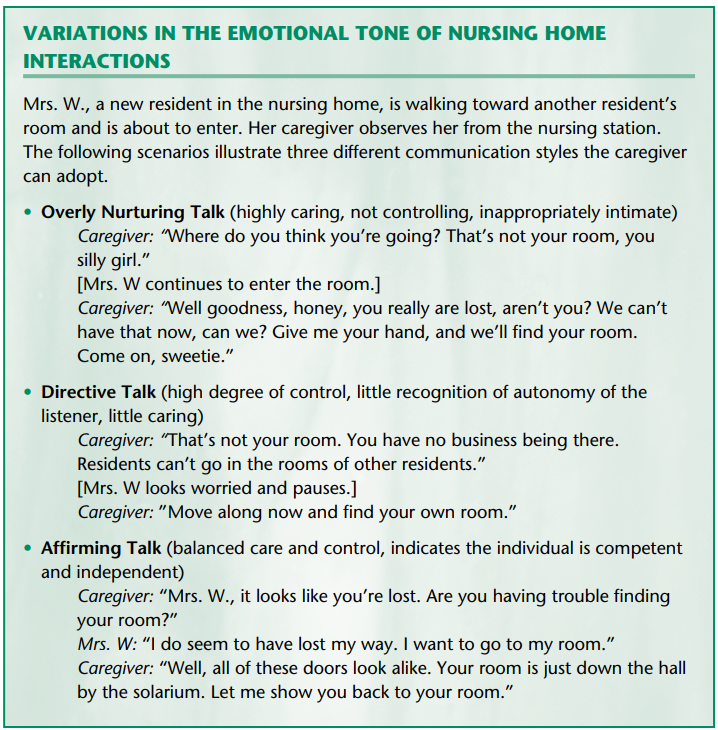
\includegraphics[width=0.5\textwidth]{enhancing_communication_with_older_adults.png}
    \captionsetup{justification=centering}
    \caption{Een Vergelijking van Communicatiedynamieken: Benaderingen van Zorgverleners met Oudere patiënten \autocite{williams2005enhancing}.}
    \label{fig:voorbeeld_affirmative_toon}
\end{figure}


\section{Vergrijzing in Vlaanderen}
%TODOEen analyse van de demografische evolutie en de gevolgen van de babyboom in de jaren '60. 

%- Toekomstige uitdagingen in de zorgsector door de vergrijzing. 

In de hedendaagse zorg- en welzijnssector is er een verschuiving zichtbaar van aanbodgestuurde naar persoonsgerichte zorg. Dit houdt in dat zorgverleners zorg op maat bieden, rekening houdend met de unieke behoeften, voorkeuren, wensen en verwachtingen van elke cliënt of patiënt. 

Persoonsgerichte zorg vereist dat zorgverleners hun communicatiestijl aanpassen aan de zorgvragers, omdat kwaliteitsvol sociaal contact essentieel is en een positieve invloed heeft op zowel de fysieke als mentale gezondheid en levenskwaliteit van zorgvragers.
Er is echter kritiek op de manier waarop communicatie vaak plaatsvindt tussen zorgverleners en zorgvragers. Deze communicatie wordt soms als ontoereikend en betuttelend beschouwd, waarbij zorgverleners specifiek voor dit onderzoek oudere patiënten, vaak een kinderlijke stijl hanteren, gekenmerkt door een overdreven toonhoogte, eenvoudige taal en het gebruik van verkleinwoorden en troetelnamen, een stijl die bekend staat als 'Secondary Babytalk' (Bron-hogent)
\\
\\
In 2023 vertoont de bevolkingspiramide van het Vlaamse Gewest het kenmerkende profiel van een vergrijzende bevolking, met een toenemend percentage van 65-plussers (21\%) ten opzichte van 2000 (17\%). Deze demografische verandering brengt nieuwe uitdagingen met zich mee in de zorgsector, met name de communicatie tussen zorgverleners en zorgbehoevenden in deze leeftijdscategorie \autocite{Vlaanderen.be}. 

%De vergrijzing van de bevolking leidt tot een toename in het aantal ouderen die zorg nodig hebben, vaak met specifieke communicatiebehoeften
%Dit kan variëren van gehoorproblemen tot cognitieve uitdagingen. Hierin ligt het belang dit mijn onderzoek: Een applicatie ontwikkelen die kenmerken van 'Secondary Babytalk' kan identificeren aan de hand van bepaalde 'Spraak-naar-tekst' modellen die beschikbaar zijn op de markt. Deze modellen zullen met elkaar vergeleken worden aan de hand van specifieke criteria. Dit zal resulteren dat het meest accurate model verkozen kan worden .
%- Elderspeak: Definitie, voorbeelden, en het belang van aangepaste communicatie met ouderen. 
\section{Artificiële Intelligentie en Automatische Spraakherkenning}

\textcite{Fetzer_1990} analyseert \gls{ai}, waarbij hij de complexiteit van het domein belicht en de uitdagingen bij het definiëren ervan bespreekt. Hij verkent de menselijke oorsprong van AI-entiteiten en de diverse aspecten van intelligentie binnen dit domein, van basisvaardigheden tot geavanceerd redeneren. Fetzer benadrukt de noodzaak van grondig onderzoek om de essentie van intelligentie in \gls{ai} te begrijpen.

\gls{ai} en \gls{asr} vormen twee essentiële componenten binnen de context van 'Elderspeak' monitoring, een cruciale praktijk in de gezondheidszorg voor oudere patiënten. Door \gls{ai} en \gls{asr} te integreren in monitoringsystemen kunnen zorgverleners effectiever communiceren met oudere patiënten, wat leidt tot verbeterde zorgkwaliteit en patiënttevredenheid.

\gls{ai} biedt geavanceerde technieken voor het analyseren en interpreteren van spraakgegevens, waardoor het mogelijk is om subtiele kenmerken en patronen in de spraak van oudere patiënten te identificeren. Dit omvat niet alleen het herkennen van woorden en zinnen, maar ook het begrijpen van de context, emoties en nuances in de spraak. Hierdoor kunnen zorgverleners beter inzicht krijgen in de behoeften en gezondheidsstatus van oudere patiënten, zelfs wanneer zij moeite hebben om zich verbaal uit te drukken \autocite{young2002,jabraf2019}.

\gls{asr} speelt een cruciale rol bij het omzetten van spraak naar tekst, waardoor gesproken informatie snel en nauwkeurig kan worden vastgelegd en geanalyseerd \autocite{rabiner1993fundamentals,jabraf2017}.

Dit stelt zorgverleners in staat om effectiever te communiceren met oudere patiënten, waarbij spraak wordt omgezet in geschreven tekst die kan worden opgeslagen, geanalyseerd en geïnterpreteerd voor verdere diagnostiek en behandeling.

\section{Communicatie in de Zorg}
Communicatie in de zorg, met name bij oudere patiënten, speelt een cruciale rol bij het leveren van effectieve en gepersonaliseerde zorg \autocite{smith2020}.

%TODO tekst van source word file (image toevoegen )
Ouderen kunnen vaak te maken hebben met verschillende gezondheidsproblemen en kunnen moeite hebben om zich duidelijk uit te drukken, waardoor communicatie met zorgverleners uitdagend kan zijn. Het is essentieel om een ​​omgeving te creëren waarin zorgverleners in staat zijn om de behoeften en zorgen van oudere patiënten effectief te begrijpen en hierop te reageren. Effectieve communicatie draagt bij aan het vergroten van de tevredenheid van patiënten, het verbeteren van behandelingsresultaten en het verhogen van de kwaliteit van de zorg.

\gls{ai} en \gls{asr} spelen een steeds grotere rol in het verbeteren van communicatieprocessen in de zorg, inclusief die met oudere patiënten \autocite{patel2019}. 

Door die twee technologieën te incorporeren in zorgsystemen kunnen zorgverleners sneller en nauwkeuriger informatie vastleggen, interpreteren en communiceren. Dit stelt hen in staat om efficiënter te werken en beter in te spelen op de behoeften van patiënten. Bovendien kunnen \gls{ai}-gebaseerde systemen zorgverleners ondersteunen bij het begrijpen van complexe spraakpatronen en het identificeren van belangrijke informatie, wat kan bijdragen aan het verbeteren van de kwaliteit en nauwkeurigheid van de communicatie \autocite{patel2019}. 
\section{Analyse van ASR-technologieën}

\subsection{Beschikbare Modellen}

\subsubsection{AssemblyAI}
AssemblyAI biedt een hoogwaardige \gls{asr}-service die specifiek is geoptimaliseerd voor een gemakkelijk ontwikkelaar ervaring en een breed scala aan talen en dialecten. 
Het is bekend om zijn robuustheid tegenover achtergrondgeluiden en biedt uitgebreide documentatie om integratie te vergemakkelijken \autocite{assemblyai2024}.

\subsubsection{Google Cloud \gls{stt} }
Google Cloud \gls{stt} maakt gebruik van geavanceerde deep learning technologieën en biedt brede taalondersteuning, inclusief voor de Nederlandse taal. De dienst kan echter relatief kostbaar zijn bij grote volumes en soms ontbreken er aanpassingsopties voor specifieke vereisten \autocite{googleasr2024}.

\subsubsection{Microsoft Azure \gls{stt}}
Microsoft Azure \gls{stt} is een flexibel \gls{asr}-systeem dat goed geïntegreerd kan worden binnen het Microsoft-ecosysteem en een ruime ondersteuning biedt voor talen, maar kan duur zijn bij grootschalige toepassingen en vereist soms aanzienlijke technische kennis voor maatwerk \autocite{azurespeech2024}.

\subsubsection{Amazon Transcribe}
Amazon Transcribe heeft uitgebreide functies voor verschillende zakelijke sectoren, met inbegrip van de gezondheidszorg en klantenservice. Echter, de kosten voor de service kunnen hoog oplopen bij veelvuldig gebruik \textcite{AmazonTranscribe2023}.

\subsubsection{Whisper}
 Whisper is een model van OpenAI die geoptimaliseerd is voor uiteenlopende accenten en presteert goed in lawaaierige omgevingen. Het is geschikt voor lange audiofragmenten en blijkt een \gls{wer} van 14.8\% voor basisschoolkinderen en 30.7\% voor middelbare scholieren te hebben bij de verwerking van Vlaamse spraak \autocite{whisper2023}.

\subsubsection{Wav2Vec 2.0}
Wav2vec-U, ontwikkeld door Facebook \gls{ai}, is een innovatieve benadering voor spraakherkenning die geen getranscribeerde gegevens vereist. Het model is vergelijkbaar met de prestaties van de best begeleide modellen van enkele jaren geleden, getraind met bijna 1000 uur aan getranscribeerde spraak. Deze methode, die spraakstructuren leert uit ongelabelde audio met behulp van een zelf-superviserend model en k-means clustering, is een belangrijke stap naar toegankelijkere spraaktechnologie voor een breed scala aan talen en dialecten \autocite{wav2vecu2021}.

\subsubsection{Hugging Face}
Hugging Face's ASR-technologie, onderdeel van de Transformers-bibliotheek, biedt uitgebreide ondersteuning voor het ontwikkelen van geavanceerde spraak-naar-teksttoepassingen. Deze technologie stelt ontwikkelaars en onderzoekers in staat om toegankelijke en efficiënte ASR-oplossingen te creëren, dankzij de mogelijkheid tot het 'fine-tuning' van modellen zoals Wav2Vec2 en de ondersteuning van een breed scala aan talen en dialecten \autocite{huggingface2023asr}.

\subsubsection{Kaldi}

Kaldi vertegenwoordigt een uitgebreid kader voor het uitvoeren van onderzoek naar spraakherkenning, waarbij een breed scala aan hulpmiddelen wordt geboden voor modellering en analyse. Ontwikkeld met als doel de ontwikkeling van robuuste en efficiënte ASR-systemen te vergemakkelijken. Kaldi onderscheidt zich door zijn ondersteuning voor lineaire algebra operaties, flexibiliteit in het modelleren van complexe spraakpatronen, en zijn open-source aard, wat samenwerking en innovaties binnen de gemeenschap van spraakherkenning aanmoedigt \autocite{Povey_ASRU2011}.


\section{Evaluatiemethoden en metrics}
\subsection{Belang van evaluatie binnen ASR}
Evaluatie van automatische spraakherkenning (ASR) systemen is essentieel 
om te begrijpen hoe goed ze presteren vanuit het perspectief van menselijke gebruikers, wat cruciaal is voor het meten van hun bruikbaarheid en het beoordelen van overgebleven uitdagingen, vooral bij het vergelijken van verschillende systemen. 

Ondanks de vooruitgang van ASR tot commercieel bruikbare toepassingen, blijft een hoge foutenmarge in sommige spraakherkenningsdomeinen een belangrijke belemmering voor de bredere adoptie van spraaktechnologie, met name voor toepassingen die continue spraakherkenning met een grote woordenschat vereisen.

De aanhoudende aanwezigheid van ASR-fouten heeft de noodzaak versterkt om alternatieve technieken te vinden voor het automatisch detecteren en corrigeren van dergelijke fouten. De correctie van transcriptiefouten is niet alleen cruciaal om de nauwkeurigheid van spraakherkenning te verbeteren, maar ook om te voorkomen dat fouten doorstromen naar volgende taalverwerkingsmodules, zoals machinevertaling \autocite{Errattahi_2018}.

Het onderzoek van \textcite{Errattahi_2018} focust op opkomende technieken die de foutenratio meten en de staat van het onderzoek naar de detectie en correctie van ASR-fouten evalueren. Automatische detectie en correctie van ASR-fouten is een belangrijk onderzoeksgebied geworden, niet alleen om de nauwkeurigheid van spraakherkenning te verbeteren, evenals het verhinderen dat fouten worden doorgegeven aan processen na herkenning, zoals machinevertaling en mens-computer interactie. Het doel is om fouten automatisch te detecteren, te classificeren en vervolgens gedeeltelijk of volledig te corrigeren, ongeacht het gebruikte ASR-systeem. Dit kan bijzonder effectief zijn, vooral wanneer het ASR-systeem wordt gebruikt als een 'black-box' waarbij de gebruiker geen toegang heeft om de kenmerken en modellen van het ASR-systeem af te stellen.

Het doel van ASR-evaluatie is om een vergelijkingscriterium te bieden tussen verschillende systemen of technieken en om de vooruitgang en prestaties op specifieke taken te meten op basis van foutenstatistieken. Er zijn twee essentiële aspecten gerelateerd aan ASR-fouten: de referentie-herkende afstemming, die het vinden van de beste woordafstemming tussen de referentie en de automatische transcriptie omvat, en de evaluatiemetrics die de prestaties van de ASR-systemen meten \autocite{McCowan2004}.


Volgens \textcite{McCowan2004} moeten de eigenschappen van een ideale evaluatiemaatstaf voor ASR als volgt zijn:
\begin{enumerate}[label=\arabic*.]
 \item \textbf{Direct:} De maatstaf meet de ASR-component onafhankelijk van de ASR-toepassing.
 
 \item \textbf{Objectief:} De maatstaf wordt op een geautomatiseerde manier berekend.
 
 \item \textbf{Interpreteerbaar:} De absolute waarde van de maatstaf geeft inzicht in de prestatie.
 
 \item \textbf{Modulair:} De evaluatiemaatstaf is algemeen genoeg om gedetailleerde toepassingsafhankelijke analyses mogelijk te maken.
\end{enumerate} 

\subsection{ASR Prestatie factoren}
ASR-prestaties worden beïnvloed door verschillende factoren, waaronder:
\begin{enumerate}[label=\arabic*.]
    \item \textbf{Sprekervariabiliteit:}
    De akoestische modellen zijn meestal gebaseerd op een beperkte hoeveelheid spraakgegevens die sprekers kenmerken op een bepaald moment en in een bepaalde situatie. Echter, de stem kan veranderen door factoren als veroudering, ziekte, emoties en vermoeidheid, waardoor het akoestische model mogelijk niet representatief is voor alle sprekers in al hun mogelijke staten.
    
    \item \textbf{Variabiliteit in gesproken taal:}
    Spontane spraak, accenten en een hoge mate van uitspraakvariatie door dialecten en articulatie vormen bekende uitdagingen voor ASR. Met een grote woordenschat wordt het bovendien steeds moeilijker om voldoende gegevens te vinden om de taalmodellen te trainen, wat vaak resulteert in het gebruik van sub-woordenmodellen in plaats van woordenmodellen, wat de prestaties aanzienlijk kan verminderen.
    
    \item \textbf{Mismatchfactoren:}
    Een van de grootste uitdagingen bij spraakherkenning komt door verschillen in opnamecondities tussen de trainings- en testfasen, vooral wanneer het spraaksignaal via telefoonlijnen wordt verkregen. 
    
    Verschillen in achtergrondgeluid, het transmissiekanaal en de opnameapparaten kunnen variabiliteit introduceren in de opnames, wat leidt tot een verminderde nauwkeurigheid van het systeem.
\end{enumerate} 


Deze factoren onderstrepen het belang van voortdurende verbetering en aanpassing van ASR-systemen om de uiteenlopende variabiliteiten en mismatchfactoren te kunnen accommoderen en daarmee de algehele systeemprestaties te verbeteren. Het onderzoek en de ontwikkeling van methoden voor het detecteren en corrigeren van ASR-fouten zijn daarom cruciaal voor het vergroten van de bruikbaarheid en acceptatie van ASR-technologieën in diverse toepassingen \autocite{Errattahi_2018}.

\subsection{ASR Fouten detectie}
In de context van automatische spraakherkenning (ASR) is de detectie van fouten een kritiek aspect dat de bruikbaarheid en intelligentie van ASR-systemen in praktische toepassingen aanzienlijk kan verbeteren \autocite{jiang2005confidence}.

Het primaire doel van foutdetectie binnen ASR-systemen, zoals uiteengezet in het onderzoek van \textcite{jiang2005confidence}, is om de betrouwbaarheid van spraak-naar-tekst conversies te verhogen door effectief fouten in transcripties te identificeren. Dit doel is van cruciaal belang omdat zelfs geavanceerde ASR-technologieën te maken hebben met een significante foutmarge als gevolg van factoren zoals achtergrondgeluid, sprekersvariatie, en de complexiteit van taal zelf.

Foutdetectiemechanismen zijn ontworpen om onnauwkeurigheden in transcripties te identificeren, waarbij onderscheid wordt gemaakt tussen verschillende soorten fouten zoals substitutie, deletie, of invoeging. Een nauwkeurige detectie van deze fouten is essentieel voor daaropvolgende correctiestrategieën, die tot doel hebben de ASR-output dichter bij de daadwerkelijk gesproken inhoud te brengen.

Verder is in het onderzoek aangegeven dat ASR-foutdetectie de basis vormt voor het verbeteren van de gebruikerservaring in applicaties die afhankelijk zijn van spraakherkenning. Door de ontwikkeling van geavanceerde technieken voor foutdetectie en -correctie kunnen ASR-systemen niet alleen accurater worden, maar ook meer geïntegreerd in een breed scala aan toepassingen, variërend van spraakgestuurde assistenten tot automatische ondertiteling \autocite{jiang2005confidence}.

\subsection{ASR Fouttypes}
Automatische spraakherkenning (ASR) heeft aanzienlijke vooruitgang geboekt, maar blijft gevoelig voor fouten die de nauwkeurigheid en bruikbaarheid beïnvloeden. Er zijn meerdere typen fouten die in ASR-systemen kunnen voorkomen, elk met specifieke oorzaken en gevolgen \autocite{Errattahi_2018}: 

\begin{enumerate}[label=\arabic*.]
    \item \textbf{Substitutiefouten:}
    treden op wanneer het ASR-systeem een verkeerd woord herkent in plaats van het gesproken woord. Dit kan te wijten zijn aan de gelijkenis in klank tussen woorden of aan de beperkte precisie van het systeem bij het onderscheiden van spraakklanken.
    
    \item \textbf{Invoegfouten:}
    worden gekenmerkt door het onjuist toevoegen van woorden die niet door de spreker zijn uitgesproken. Deze fouten kunnen ontstaan door achtergrondgeluiden of door het systeem dat ten onrechte pauzes of geluiden interpreteert als woorden.
    
    \item \textbf{Verwijderfouten:}
    ontstaan wanneer het ASR-systeem een gesproken woord niet detecteert of herkent, waardoor dit woord afwezig is in de transcriptie. Dit kan het gevolg zijn van een lage spreeksnelheid, articulatieproblemen of wanneer het spraaksignaal wordt gemaskeerd door achtergrondlawaai.   
\end{enumerate}

Het verbeteren van de nauwkeurigheid van ASR en het verminderen van deze fouten vereist geavanceerde technieken, data-augmentatie en robuuste akoestische modellen die beter bestand zijn tegen variabiliteit in spraak en opnameomstandigheden \autocite{Errattahi_2018}.

Ondanks deze uitdagingen biedt ASR enorme mogelijkheden voor toepassingen variërend van spraakgestuurd assistenten tot automatische ondertiteling, wat de motivatie vormt voor voortdurend onderzoek en ontwikkeling in dit veld \autocite{Errattahi_2018}.

\subsection{Word Error Rate (WER)}
Automatische spraakherkenningssystemen (ASR) hebben de afgelopen tien jaar aanzienlijke vooruitgang geboekt, waarbij de Word Error Rate (WER) naar voren is gekomen als de voornaamste maatstaf voor het evalueren van de prestaties van deze systemen \autocite{Raghavan2022}.

WER is gebaseerd op het concept van de bewerkingsafstand en kwantificeert de nauwkeurigheid van ASR door de verhouding van invoegingen, verwijderingen en vervangingen ten opzichte van het totale aantal tokens in een zin te berekenen. Deze maatstaf is bijzonder effectief voor talen zoals het Engels, die doorgaans één spelling voor elk woord hebben, waardoor WER de algehele correctheid nauwkeurig kan weerspiegelen door de getranscribeerde tekst te vergelijken met de oorspronkelijke spraak \autocite{Raghavan2022}.



\begin{equation}
    WER(w) = \frac{i + d + s}{N_t}
\end{equation}
waarbij:
\begin{itemize}
    \item \(i\) Is het aantal invoegingen.
    \item \(d\) Is het aantal verwijderingen.
    \item \(s\) Is het aantal substituties.
    \item \(N\) Is de totale aantal woorden.
\end{itemize}

\begin{figure}[h]
    \centering
    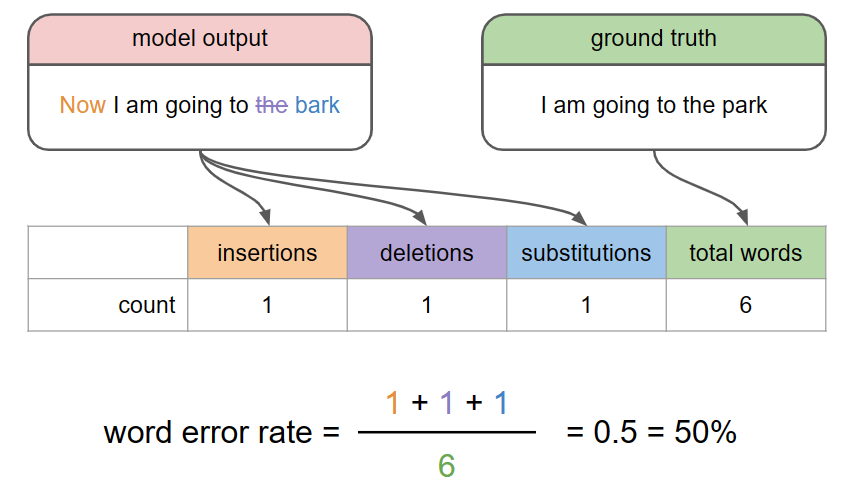
\includegraphics[width=0.5\textwidth]{ryan_oconor.png}
    \captionsetup{justification=centering}
    \caption{Berekening van WER voor een voorbeeldmodeloutput gegeven de grondwaarheid transcriptie \autocite{OConnor2023}.}
    \label{fig:voorbeeld}
\end{figure}

\subsection{Beperkingen van WER}
 Ondanks het wijdverbreide gebruik van WER als een standaardmaat voor de prestaties van ASR-systemen, identificeert het onderzoek enkele belangrijke beperkingen van deze maatstaf. De studie van \textcite{Kwint2023} benadrukt dat WER niet als een absoluut percentage kan worden beschouwd vanwege het ontbreken van een bovengrens. 
 
 Dit impliceert dat WER alleen kan aangeven dat het ene systeem beter presteert dan het andere, maar niet noodzakelijkerwijs hoe goed een systeem absoluut is. Daarnaast is WER niet symmetrisch ten aanzien van deleties en invoegingen, waardoor het in lawaaierige omstandigheden meer dan 100\% kan overschrijden door een onevenredige nadruk op invoegingen vergeleken met verwijderingen. Het onderzoek toont aan dat, hoewel WER effectief blijft voor toepassingen zoals dicteren waar fouten handmatig gecorrigeerd kunnen worden, er voor de meeste andere soorten spraakherkenningssystemen, waarbij het doel verder gaat dan louter transcriptie, behoefte is aan alternatieve of aanvullende evaluatiekaders. Dit is vooral relevant in domeinen zoals geautomatiseerde medische rapportage, waar de nauwkeurigheid van de transcriptie directe gevolgen kan hebben voor de kwaliteit van de patiëntenzorg \autocite{Kwint2023}.

Door het analyseren van bestaande medische audio-data en het uitvoeren van een pilot-experiment, onderzoekt deze studie de invloed van elementen zoals accent, stemfrequentie en omgevingslawaai op de kwaliteit van ASR-transcripties. De resultaten wijzen op de significante impact van lawaai op de WER, hoewel het experiment door een beperkt aantal deelnemers geen significante verschillen kon aantonen. Dit onderstreept het belang van verder onderzoek naar de effecten van lawaai, taal en verschillende ASR-technologieën op de nauwkeurigheid van spraakherkenning, vooral in kritieke toepassingen zoals medische rapportage.

Het gebruik van de Woord Fout Ratio (WER) als enige maatstaf voor de evaluatie van spraakherkenningssystemen blijkt beperkt. Hoewel WFR een indicatie geeft van de algemene prestaties, mist het nuances, vooral met betrekking tot disfluenties zoals vulwoorden ("uh", "um"). Deze aspecten van spraak, die de denkprocessen van de spreker weerspiegelen, kunnen waardevol zijn voor de ene context maar overbodig voor de andere \textcite{Kwint2023}.
\\
\\
Een discrepantie tussen de transcriptie van disfluenties door het model en de ‘grondwaarheid’ transcriptie kan leiden tot een onnauwkeurige WER. Daarom pleit deze analyse voor een evaluatiemethode die rekening houdt met de complexiteit en contextuele afhankelijkheid van spraak, wat zou resulteren in een accurater en relevanter beoordeling van spraakherkenningssystemen \autocite{OConnor2023}.

\begin{figure}[h]
    \centering
    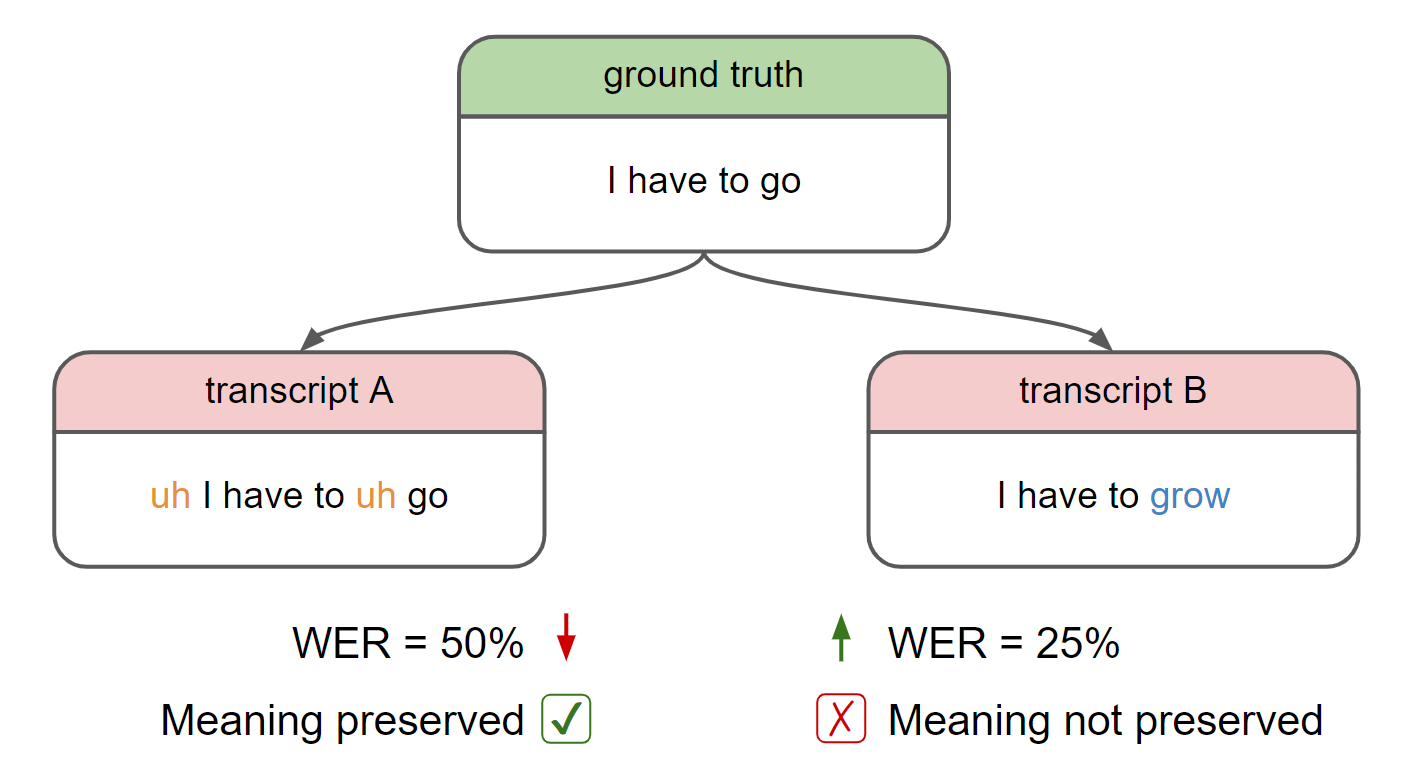
\includegraphics[width=0.5\textwidth]{ryan_oconor_meaning.png}
    \captionsetup{justification=centering}
    \caption{Voorbeeld van een onnauwkeurige WER resultaat \autocite{OConnor2023}.}
    \label{fig:voorbeeld}
\end{figure}

\subsection{Jaro-Winkler Afstand (JW)}
De Jaro-Winkler-afstand is een algoritme dat in twee delen is opgedeeld. Het eerste deel, de Jaro-implementatie, houdt rekening met de overeenkomende karakters tussen twee strings, ongeacht de volgorde. Als de overeenkomende karakters in een andere volgorde staan, wordt een tolerantievenster gebruikt voor het aantal transposities. De Jaro-Winkler afstand wordt berekend met een formule die de overeenkomsten en transposities tussen de strings in acht neemt, waarbij gewichten kunnen worden toegepast om de invloed van verschillende factoren te moduleren \autocite{Rdazzi2023comparison}.

Het tweede deel, de Winkler-aanpassing, verbetert de Jaro-score door extra gewicht toe te kennen aan strings die in de begin karakters overeenkomen. Dit reflecteert het idee dat overeenkomsten aan het begin van de strings belangrijker zijn voor de totale perceptie van gelijkenis tussen strings. De Jaro-Winkler-afstand wordt dan berekend door aanpassingen aan de oorspronkelijke Jaro-score toe te voegen op basis van de overeenkomst aan het begin van de strings en de totale lengte van de strings \autocite{Rdazzi2023comparison}.

De \(JW\) tussen twee woorden \(X\) en \(Y\) kan berekend worden als volgt:
\begin{equation}
    JW = \frac{1}{3} \left( \frac{m}{\text{lengte}(X)} + \frac{m}{\text{lengte}(Y)} + \frac{m - t}{m} \right)
\end{equation}

Waarbij:
\begin{itemize}
    \item \(m\) Is het aantal overeenkomsten.
    \item \(t\) Is het aantal transposities.
\end{itemize}


\subsection{Character Error Rate (CER)}
Het karakterfoutpercentage (CER) biedt een gedetailleerde methode voor het evalueren van automatische spraakherkenningsystemen (ASR) door de prestaties op karakterniveau te beoordelen, in tegenstelling tot het woordfoutpercentage (WER), dat beoordelingen op woordniveau uitvoert. CER is vooral nuttig in talen zonder duidelijke woordgrenzen of in situaties waar nauwkeurigheid op karakterniveau cruciaal is. 
Hoewel WER veel gebruikt wordt voor een alomvattende beoordeling in veel talen, maakt CER gerichte verbeteringen in ASR-systemen mogelijk, waardoor het een cruciale rol speelt in linguïstische en technische toepassingen die hoge nauwkeurigheid vereisen \autocite{huggingface2023asr}.

\begin{equation}
    CER = \frac{S + D + I}{N}
\end{equation}
Waarbij:
\begin{itemize}
    \item $S$ Het aantal substitutiefouten.
    \item $D$ Het aantal verwijderingsfouten.
    \item $I$ Het aantal invoegfouten.
    \item $N$ Het totale aantal karakters in de referentie.
\end{itemize}

\subsection{Het belang van sampeling en data verzameling}
Bij het evalueren van Automatische Spraakherkenning (ASR) systemen is het kiezen van de juiste monsters essentieel voor een nauwkeurige beoordeling. Het proces omvat de volgende stappen \autocite{awsmlblog2023}:

\begin{enumerate}
    \item Kies een kleine steekproef van opgenomen spraak, zorgend voor diversiteit en representativiteit.
    \item Transcribeer de monsters handmatig om referentietranscripten te maken.
    \item Verwerk deze monsters door de ASR-service.
    \item Normaliseer de door ASR gegenereerde hypothese transcripten voor consistentie.
    \item Bereken de Word Error Rate (WER) met een open-source tool.
    \item Maak beoordelingen op basis van relevante metrieken.
\end{enumerate}

Het is belangrijk om uitspraken zorgvuldig te selecteren om vooringenomenheid te vermijden en een verscheidenheid aan spraakcontexten op te nemen, zoals verschillende geluidsniveaus, sprekers en accenten \autocite{awsmlblog2023}.


Zowel wanneer het gaat om het evalueren van automatische spraakherkennings (ASR) systemen als in andere onderzoeksgebieden, spelen steekproeftechnieken een cruciale rol. Hierbij worden verschillende methoden toegepast om ervoor te zorgen dat de verzamelde gegevens een nauwkeurige representatie vormen van de diversiteit aan spraakpatronen en omgevingsomstandigheden die in de echte wereld worden aangetroffen \autocite{huggingface2023asr}:
\begin{enumerate}[label=\arabic*.]
 
    \item \textbf{Willekeurige Steekproef:}
        Bij willekeurige steekproeven worden voorbeelden willekeurig geselecteerd uit de gehele populatie van belang.Dit zorgt ervoor dat alle spraakpatronen en omgevingsomstandigheden een gelijke kans krijgen om te worden opgenomen in het evaluatie dataset.
        
    \item \textbf{Gestratificeerde Steekproef:}
        Gestratificeerde steekproeven verdelen de populatie in subgroepen op basis van criteria zoals sprekerskenmerken of omgevingsfactoren. Voorbeelden worden willekeurig geselecteerd uit elke subgroep, wat een evenredige vertegenwoordiging garandeert. Dit maakt gerichte evaluatie van ASR-prestaties mogelijk over verschillende demografische of omgevingsfactoren.
        
    \item \textbf{Clustersteekproef:}
        Clustersteekproeven verdelen de populatie in clusters, zoals geografische regio's of organisatorische eenheden, waarbij willekeurig clusters worden gekozen voor evaluatie. Binnen elk cluster worden alle monsters of een willekeurige subset ervan opgenomen. Hoewel handig voor natuurlijk gegroepeerde populaties, kan dit leiden tot minder diversiteit als er grote variaties tussen clusters zijn.
         
\end{enumerate}


%- Inleiding tot Evaluatiemethoden: Het belang van evaluatie in ASR. 
%- Word Error Rate (WER): Basisconcept en beperkingen. 
%- Beyond WER: Geavanceerdere evaluatiemethoden voor een completere beoordeling. 
%- Evaluatie van Eigennamen en Specifieke Datasets: Het belang van nauwkeurigheid bij eigennamen en specifieke terminologie. 
%- Bias en Diversiteit in Datasets: Uitdagingen en oplossingen voor bias en het waarborgen van diversiteit.  

\section{Beschikbaar ASR evaluatie tools}
\subsection{JIWER (Jitsi Word Error Rate):} JIWER vertegenwoordigt een efficiënte en gebruikersvriendelijke Python-bibliotheek, specifiek ontworpen voor het evalueren van prestaties van automatische spraakherkenningsystemen (ASR). Dit instrument faciliteert de kwantitatieve beoordeling van ASR-modellen door middel van diverse nauwkeurigheidsmetrieken, die cruciaal zijn voor het begrijpen en verbeteren van de betrouwbaarheid van spraak-naar-tekst conversies \autocite{jiwer2023}.

\subsection{Speech Recognition Evaluation:} De "Speech Recognition Evaluation" tool van Symbl.AI is een geavanceerde en toegankelijke hulpmiddel voor iedereen die werkt met spraak-naar-tekst of spraakherkenningssystemen. Deze tool stelt gebruikers in staat om de nauwkeurigheid van automatische transcripties, gegenereerd door spraakherkenningssoftware, te vergelijken met transcripties gemaakt door mensen. Dit is cruciaal voor ontwikkelaars, onderzoekers, en gebruikers die de prestaties van hun spraak-naar-tekstsystemen willen evalueren en verbeteren \autocite{speechrecognitionevaluation2021}.

\section{Persoonlijke Bijdrage en Toekomstvisie}

In mijn onderzoek richt ik mij op het evalueren van spraak-naar-tekst modellen met als doel de transcriptie van 'Secondary Babytalk' te verbeteren voor nauwkeurigere communicatie binnen de zorgsector. Dit streven naar grotere accuratesse in transcripties is essentieel om misverstanden te voorkomen en de dialoog tussen zorgverleners en oudere patiënten te optimaliseren. Door de meest effectieve modellen te identificeren en toe te passen, beoog ik een significante verbetering in de kwaliteit van zorgcommunicatie te realiseren. Daarnaast zal er een Proof of Concept (POC) worden geïmplementeerd die het geselecteerde model zal adapteren en gebruiken voor transcriptie doeleinden.


%Dit hoofdstuk bevat je literatuurstudie. De inhoud gaat verder op de inleiding, maar zal het onderwerp van de bachelorproef *diepgaand* uitspitten. De bedoeling is dat de lezer na lezing van dit hoofdstuk helemaal op de hoogte is van de huidige stand van zaken (state-of-the-art) in het onderzoeksdomein. Iemand die niet vertrouwd is met het onderwerp, weet nu voldoende om de rest van het verhaal te kunnen volgen, zonder dat die er nog andere informatie moet over opzoeken \autocite{Pollefliet2011}.
%Je verwijst bij elke bewering die je doet, vakterm die je introduceert, enz.\ naar je bronnen. In \LaTeX{} kan dat met het commando \texttt{$\backslash${textcite\{\}}} of \texttt{$\backslash${autocite\{\}}}. Als argument van het commando geef je de ``sleutel'' van een ``record'' in een bibliografische databank in het Bib\LaTeX{}-formaat (een tekstbestand). Als je expliciet naar de auteur verwijst in de zin (narratieve referentie), gebruik je \texttt{$\backslash${}textcite\{\}}. Soms is de auteursnaam niet expliciet een onderdeel van de zin, dan gebruik je \texttt{$\backslash${}autocite\{\}} (referentie tussen haakjes). Dit gebruik je bv.~bij een citaat, of om in het bijschrift van een overgenomen afbeelding, broncode, tabel, enz. te verwijzen naar de bron. In de volgende paragraaf een voorbeeld van elk.

%\textcite{Knuth1998} schreef een van de standaardwerken over sorteer- en zoekalgoritmen. Experten zijn het erover eens dat cloud computing een interessante opportuniteit vormen, zowel voor gebruikers als voor dienstverleners op vlak van informatietechnologie~\autocite{Creeger2009}.

%Let er ook op: het \texttt{cite}-commando voor de punt, dus binnen de zin. Je verwijst meteen naar een bron in de eerste zin die erop gebaseerd is, dus niet pas op het einde van een paragraaf.


%%=============================================================================
%% Methodologie
%%=============================================================================

\chapter{\IfLanguageName{dutch}{Methodologie}{Methodology}}%
\label{ch:methodologie}

Dit hoofdstuk biedt een gestructureerd overzicht van de methodologische aanpak die is gehanteerd in dit onderzoek. Het is bedoeld om de lezer inzicht te geven in de onderzoeksopzet, de gehanteerde methoden en de rationale achter de gekozen aanpak. Het onderzoek is opgedeeld in verschillende fasen, elk met specifieke doelstellingen, deliverables, en onderzoeksmethoden. De onderstaande secties beschrijven deze fasen in detail.

%Literatuurstudie
De eerste fase van het onderzoek bestond uit een uitgebreide literatuurstudie, gericht op het verkennen van het bestaande kennisdomein met betrekking tot 'secondary babytalk', de beschikbare spraak-naar-tekst (ASR) modellen, en de criteria voor model evaluatie. Deze fase had als doelstelling het vaststellen van een theoretische basis voor het onderzoek.

%Selectie van ASR Modellen

In de literatuurstudie kwam een fase waarbij bepaalde ASR modellen uitgekozen werden voor een analyse. De keuze voor deze modellen was gebaseerd op de beschikbaarheid en ondersteuning van het Vlaamse en Nederlandse taal. Die modellen zullen dan gebruikt worden om de steekproefneming te transcriberen.



De volgende stap in het proces is het verzamelen van audio samples. Deze samples zullen vervolgens worden onderworpen aan de geselecteerde AI-modellen voor transcribering. Het doel is om elke sample te laten transcriberen door de AI-modellen. 
De resulterende transcribties, samen met de grondwaarheid 'Ground truth' transcribties, worden vervolgens gebruikt als parameters voor de Jiwer-bibliotheek om de relevante metrics te berekenen. Een diagram in figuur \ref{fig:plan_methodologie} toont de wijze waarop de evaluatieprocedure zal worden uitgevoerd.
\\

Na het verzamelen van de resultaten van deze evaluatie, worden ze samengebracht en overzichtelijk gepresenteerd in een tabel. Deze tabel zal een gedetailleerd inzicht bieden in de prestaties van de AI-modellen op basis van verschillende metrics en criteria. 

\begin{figure}[h]
    \centering
    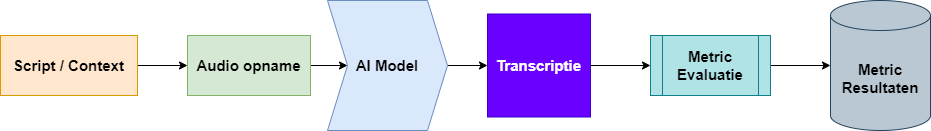
\includegraphics[width=0.8\textwidth]{plan.png}
    \captionsetup{justification=centering}
    \caption{Het uitvoeringsplan voor de evaluatieprocedure.}
    \label{fig:plan_methodologie}
\end{figure}


Ten slotte zal er op basis van de analyse van de resultaten een beslissing worden genomen. Deze beslissing kan betrekking hebben op verdere optimalisatie van de AI-modellen, het identificeren van zwakke punten in het systeem, of het bepalen van de geschiktheid van de AI-modellen voor het beoogde gebruiksscenario.


%% TODO: In dit hoofstuk geef je een korte toelichting over hoe je te werk bent
%% gegaan. Verdeel je onderzoek in grote fasen, en licht in elke fase toe wat
%% de doelstelling was, welke deliverables daar uit gekomen zijn, en welke
%% onderzoeksmethoden je daarbij toegepast hebt. Verantwoord waarom je
%% op deze manier te werk gegaan bent.
%% 
%% Voorbeelden van zulke fasen zijn: literatuurstudie, opstellen van een
%% requirements-analyse, opstellen long-list (bij vergelijkende studie),
%% selectie van geschikte tools (bij vergelijkende studie, "short-list"),
%% opzetten testopstelling/PoC, uitvoeren testen en verzamelen
%% van resultaten, analyse van resultaten, ...
%%
%% !!!!! LET OP !!!!!
%%
%% Het is uitdrukkelijk NIET de bedoeling dat je het grootste deel van de corpus
%% van je bachelorproef in dit hoofstuk verwerkt! Dit hoofdstuk is eerder een
%% kort overzicht van je plan van aanpak.
%%
%% Maak voor elke fase (behalve het literatuuronderzoek) een NIEUW HOOFDSTUK aan
%% en geef het een gepaste titel.



% Voeg hier je eigen hoofdstukken toe die de ``corpus'' van je bachelorproef
% vormen. De structuur en titels hangen af van je eigen onderzoek. Je kan bv.
% elke fase in je onderzoek in een apart hoofdstuk bespreken.

%\input{...}
%\input{...}
%...

%%=============================================================================
%% Conclusie
%%=============================================================================

\chapter{Conclusie}%
\label{ch:conclusie}

% TODO: Trek een duidelijke conclusie, in de vorm van een antwoord op de
% onderzoeksvra(a)g(en). Wat was jouw bijdrage aan het onderzoeksdomein en
% hoe biedt dit meerwaarde aan het vakgebied/doelgroep? 
% Reflecteer kritisch over het resultaat. In Engelse teksten wordt deze sectie
% ``Discussion'' genoemd. Had je deze uitkomst verwacht? Zijn er zaken die nog
% niet duidelijk zijn?
% Heeft het onderzoek geleid tot nieuwe vragen die uitnodigen tot verder 
%onderzoek?


Op basis van de gedetailleerde evaluatie en vergelijking van verschillende spraak-naar-tekstmodellen (ASR) binnen dit onderzoek, gericht op hun vermogen om diverse Belgische accenten te transcriberen, heeft men in dit onderzoek kunnen constateren dat het AssemblyAI-model uitblinkt in zowel nauwkeurigheid als consistentie. Deze conclusie steunt op gevestigde metrieken zoals de Word Error Rate (WER), Match Error Rate (MER), en Character Error Rate (CER), die allemaal zijn geïntegreerd in de JIWER-bibliotheek.

De analyse van de dataset toont aan dat AssemblyAI consistent lagere WER-scores behaalt over verschillende steekproeven heen. Bijzonder in steekproef 5, scoort AssemblyAI aanzienlijk lager dan andere modellen met een WER van slechts 0.20, wat wijst op een superieure prestatie in het correct decoderen en transcriberen van spraak. De uitmuntendheid van AssemblyAI wordt verder onderstreept door zijn prestaties op andere belangrijke metrieken zoals WIL (Word Information Lost) en WIP (Word Information Preserved), waar het consequent beter scoort dan de concurrentie, wat bijdraagt aan zijn aanbeveling voor praktische implementatie.

De consistentie van het model, zelfs in de aanwezigheid van diverse accentvariaties, illustreert de robuustheid ervan voor gebruik in kritische toepassingen, zoals de monitoring van 'Secondary Babytalk' in zorginstellingen. Dit is van cruciaal belang, omdat een accurate en betrouwbare transcriptie direct de kwaliteit van communicatie en daarmee de zorg verbetert.

Deze bevindingen benadrukken het belang van een gedegen selectieproces van spraak-naar-tekstmodellen, vooral als deze ingezet worden in kritische zorgtoepassingen waarbij elke verbetering in communicatie direct bijdraagt aan de kwaliteit van leven van de patiënten. Het vermogen van AssemblyAI om consequent hoog te scoren op verschillende metrieken ondersteunt de keuze voor dit model als de beste optie voor het ondersteunen van communicatie met oudere patiënten binnen het Belgische dialectlandschap. 
\section{Discussie}

\subsection{Beperkingen van het Onderzoek}

Ondanks dat de uitkomsten van dit onderzoek positief zij, zijn er enkele beperkingen die de algemene conclusies kunnen beïnvloeden. Ten eerste is de steekproefomvang relatief beperkt, wat de algemene toepasbaarheid van de bevindingen kan inperken. De focus was voornamelijk gericht op vier specifieke Belgische accenten en één algemene Nederlandse steekproef; de prestaties van de geteste modellen in andere dialectische en linguïstische contexten zijn daarom niet onderzocht. Dit beperkt de mogelijkheid om de resultaten te generaliseren naar andere taalvariaties.

Ten tweede was de variabiliteit in spraakcomplexiteit tussen de verschillende samples niet volledig gecontroleerd, wat suggereert dat sommige resultaten mogelijk beïnvloed zijn door verschillen in eenvoud of complexiteit van het taalgebruik. Daarnaast, hoewel AssemblyAI uitstekende resultaten liet zien, is de transparantie omtrent de parameters en training van het model niet volledig, wat vragen oproept over de reproduceerbaarheid van de studie.

Ten derde zijn de gebruikte opnames uitsluitend gemaakt in een stille omgeving. Dit aspect kan de uiteindelijke resultaten beïnvloeden wanneer er achtergrondgeluid aanwezig is tijdens de opnames. Het is daarom raadzaam om in toekomstig onderzoek ook de invloed van achtergrondgeluid op de prestaties van spraak-naar-tekstmodellen te onderzoeken.

Deze beperkingen suggereren dat verdere studies noodzakelijk zijn om de robuustheid en toepasbaarheid van de bevindingen te verifiëren, vooral in gevarieerde en realistische luisteromgevingen.
 
\subsection{Aanbevelingen voor Toekomstig Onderzoek}

Voor toekomstig onderzoek zou het waardevol zijn om de steekproefomvang te vergroten en meer diverse accentpatronen op te nemen om de robuustheid van de spraak-naar-tekstmodellen verder te testen.

 Het zou ook nuttig zijn om een diepgaandere analyse uit te voeren van de soorten fouten die door de modellen worden gemaakt, om waardevolle feedback te verkrijgen. 
 
 Deze feedback zou onderzoek kunnen ondersteunen dat gericht is op het verfijnen van algoritmen met geavanceerdere machineleertechnieken, zoals deep learning, om de nauwkeurigheid te verbeteren en een betere generalisatie over verschillende soorten spraakgegevens te waarborgen. 
 
 Deze vooruitgang zou de inzetbaarheid van deze technologieën aanzienlijk verbeteren in een breder scala van zorginstellingen.
\\
Verder heeft het onderzoek geleid tot nieuwe onderzoeksvragen die aanzetten tot verdere studies:





\begin{enumerate}[label=\arabic*.]
    
    \item Hoe zouden de modellen presteren als de opnamen willekeurig in een lawaaierige omgeving worden gemaakt ?
    \item Hoe zouden de modellen presteren als de opnames langer duren en complexere accenten bevatten?
    \item Kan het gekozen model verfijnd worden om een perfecte transcriptie te leveren?
    
\end{enumerate}





%---------- Bijlagen -----------------------------------------------------------

\appendix

\chapter{Onderzoeksvoorstel}

Het onderwerp van deze bachelorproef is gebaseerd op een onderzoeksvoorstel dat vooraf werd beoordeeld door de promotor. Dat voorstel is opgenomen in deze bijlage.

%% TODO: 
%\section*{Samenvatting}

% Kopieer en plak hier de samenvatting (abstract) van je onderzoeksvoorstel.

% Verwijzing naar het bestand met de inhoud van het onderzoeksvoorstel
%---------- Inleiding ---------------------------------------------------------

\section{Introductie}%
\label{sec:introductie}

In de hedendaagse zorg- en welzijnssector is er een verschuiving zichtbaar van aanbodgestuurde naar persoonsgerichte zorg. Dit houdt in dat zorgverleners zorg op maat bieden, rekening houdend met de unieke behoeften, voorkeuren, wensen en verwachtingen van elke cliënt of patiënt. Persoonsgerichte zorg vereist dat zorgverleners hun communicatiestijl aanpassen aan de zorgvragers, omdat kwaliteitsvol sociaal contact essentieel is en een positieve invloed heeft op zowel de fysieke als mentale gezondheid en levenskwaliteit van zorgvragers.
Er is echter kritiek op de manier waarop communicatie vaak plaatsvindt tussen zorgverleners en zorgvragers. Deze communicatie wordt soms als ontoereikend en betuttelend beschouwd, waarbij zorgverleners specifiek voor dit onderzoek oudere patiënten, vaak een kinderlijke stijl hanteren, gekenmerkt door een overdreven toonhoogte, eenvoudige taal en het gebruik van verkleinwoorden en troetelnamen, een stijl die bekend staat als 'secondary babytalk'.

In 2023 vertoont de bevolkingspiramide van het Vlaamse Gewest het kenmerkende profiel van een vergrijzende bevolking, met een toenemend percentage van 65-plussers (21\%) ten opzichte van 2000 (17\%). Dit demografische verandering brengt nieuwe uitdagingen met zich mee in de zorgsector, met name wat betreft de communicatie tussen zorgverleners en zorgbehoevenden in deze leeftijdscategorie.

De vergrijzing van de bevolking leidt tot een toename in het aantal ouderen die zorg nodig hebben, vaak met specifieke communicatiebehoeften. Dit kan variëren van gehoorproblemen tot cognitieve uitdagingen. Hierin ligt het belang dit mijn onderzoek: Een applicatie ontwikkelen die kenmerken van ‘secondary babytalk’ kan identificeren aan de hand van bepaalde speech-to-text modellen die beschikbaar zijn op de markt. Deze modellen zullen met elkaar vergeleken worden aan de hand van specifieke criteria. Dit zal resulteren dat het meest accurate model verkozen kan worden
\textcite{Vlaanderen.be}.

%---------- Stand van zaken ---------------------------------------------------

\section{State-of-the-art}%
\label{sec:state-of-the-art}
\subsection{Probleemstelling}
\begin{quote}
   `` Hoe kunnen we spraak-naar-tekstmodellen evalueren om te bepalen welk model optimaal presteert voor de specifieke usecase van spraaktranscriptie, met als doel het identificeren en verminderen van 'secondary babytalk' in een-op-een gesprekken tussen zorgverleners en oudere zorgvragers binnen de Vlaamse zorgsector, streven naar een respectvolle en doeltreffende communicatie te bevorderen?''

\end{quote}

Om deze onderzoeksvraag te kunnen beantwoorden, is een systematische aanpak vereist.

Daarvoor moet een literatuurstudie worden uitgevoerd. In deze context dienen begrippen gedefinieerd te worden. Allereerst moet beschreven worden wat een speech-to-text model precies inhoudt en waar het zich bevindt in de wereld van kunstmatige intelligentie. Welke modellen zijn beschikbaar op de markt? En wat zijn de criteria om deze modellen te testen?

\subsection{Spraak-naar-tekst}

Het begrijpen van de nuances tussen termen zoals spraakherkenning, stemherkenning en natuurlijke taalverwerking kan uitdagend zijn. In de loop van mijn onderzoek heb ik een mogelijke verduidelijking geïdentificeerd voor deze conceptuele complexiteit.

\autocite{IBM} defineert het als volgt: \\Spraakherkenning, ook wel bekend als automatische spraakherkenning (ASR), computergestuurde spraakherkenning of spraak-naar-tekst, is een functie die een programma in staat stelt menselijke spraak te verwerken en om te zetten in geschreven tekst. Hoewel het vaak verward wordt met stemherkenning, richt spraakherkenning zich op de vertaling van spraak van een verbale vorm naar een tekstuele, terwijl stemherkenning alleen probeert de stem van een individuele gebruiker te identificeren.

Spraakherkenningsmodellen produceren een transcript van spraak in audiogegevens. Dit transcript kan op zichzelf worden gebruikt of verder worden verwerkt voor andere doeleinden, zoals het gebruik van grote taalmodellen om de inhoud van de spraak te analyseren \autocite{OConnor2023}.

Samengevat Spraakherkenning, ook bekend als automatische spraakherkenning (ASR), is de mogelijkheid van een programma om gesproken taal om te zetten naar geschreven tekst.

\subsection{Beschikbaar modellen}
\subsubsection{Google Speech to Text}

Google Cloud Speech-to-Text is een API van Google Cloud Platform die gesproken taal omzet in geschreven tekst. Het ondersteunt verschillende talen, real-time streaming en batchverwerking. Gebruikers kunnen de service aanpassen voor domeinspecifieke termen en het integreert naadloos met andere Google Cloud-services. De API biedt veilige en nauwkeurige spraakherkenning voor verschillende toepassingen.\autocite{DocsGoogle}
\subsubsection{AssemblyAI}
Samengesteld door AI-experts, omvatten de spraak-AI-modellen van AssemblyAI nauwkeurige spraak-naar-tekst voor spraakgegevens (zoals gesprekken, virtuele vergaderingen en podcasts), sprekerdetectie, sentimentanalyse, hoofdstukdetectie, PII-verwijdering en meer \autocite{DocsAssemblyai}.
\subsection{Criteria}
%----------TODO THIS NEED TO BE REVIEWED 
Uiteindelijk komt een juiste evaluatie neer op het aannemen van een wetenschappelijke benadering om ervoor te zorgen dat de resultaten accuraat, herhaalbaar en betrouwbaar zijn. Laten we nu onderzoeken hoe kunnen de gekozen modellen getest worden.

\subsubsection{Word Error Rate (WER)}
Automatische spraakherkenningssystemen (ASR) hebben de afgelopen tien jaar aanzienlijke vooruitgang geboekt, waarbij de Word Error Rate (WER) naar voren is gekomen als de voornaamste maatstaf voor het evalueren van de prestaties van deze systemen. WER is gebaseerd op het concept van de bewerkingsafstand en kwantificeert de nauwkeurigheid van ASR door de verhouding van invoegingen, verwijderingen en vervangingen ten opzichte van het totale aantal tokens in een zin te berekenen. Deze maatstaf is bijzonder effectief voor talen zoals het Engels, die doorgaans één spelling voor elk woord hebben, waardoor WER de algehele correctheid nauwkeurig kan weerspiegelen door de getranscribeerde tekst te vergelijken met de oorspronkelijke spraak.\\
\autocite{Raghavan2022}.
\\De \(WER\) kan berekend worden als volgt:

\begin{equation}
   WER(w) = \frac{i + d + s}{N_t}
\end{equation}
waarbij:
\begin{itemize}
    \item \(i\) is het aantal invoegingen
    \item \(d\) is het aantal verwijderingen
    \item \(s\) is het aantal substituties
    \item \(N\) is de totale aantal woorden
\end{itemize}

In het bijzonder telt WER inserties, waarbij het model een woord transcribeert dat niet aanwezig is, verwijderingen, waarbij het model een woord dat aanwezig is niet transcribeert en substituties, waarbij het model een woord onjuist transcribeert
\autocite{OConnor2023}.
\begin{figure}[htbp]
    \centering
    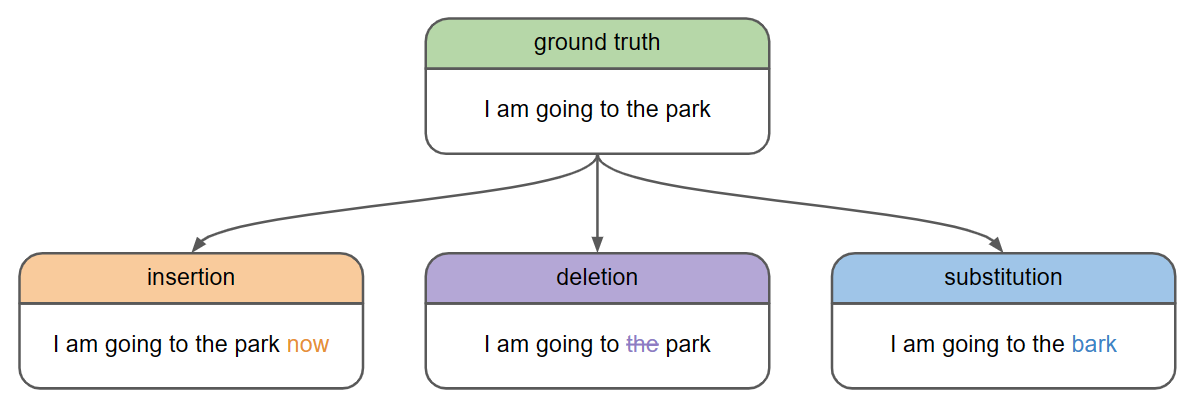
\includegraphics[width=0.5\textwidth]{wer_1}
    \caption{Een referentietranscript samen met één voorbeeld van elk van de 3 soorten fouten die WER telt \autocite{OConnor2023}.}
    \label{fig:WER count}
\end{figure}

WER wordt beïnvloed door verschillende factoren, waaronder technische taal, branchespecifieke termen, accenten en ruis in de audiogegevens. Het herkennen van technische en gespecialiseerde taal vereist extra inspanning, terwijl accenten en diverse audiogegevens mogelijk aangepaste modellen nodig hebben voor nauwkeurige transcriptie. De aanwezigheid van ruis, veelvoorkomend in real-world scenario's zoals telefoongesprekken en diverse omgevingen, vormt een uitdaging voor de nauwkeurigheid van spraakherkenningssystemen \autocite{Gevirtz2018}.

Echter zou WER alleen voldoende zijn als criterium omdat het fouten berekent op hetzelfde niveau, maar omdat het wat vaak niet het geval is moeten we een andere metriek introduceren \autocite{OConnor2023}.
\subsubsection{Jaro–Winkler distance (JW)}


De Jaro-Winkler Distance is een algoritme voor het meten van de gelijkenis tussen twee teksten en wordt voornamelijk gebruikt op het gebied van duplicatiedetectie. Dit algoritme is gebaseerd op het Jaro-Distance algoritme, dat is ontwikkeld door Matthew A. Jaro en later verder ontwikkeld door William E. Winkler en Thibaudeau door de Jaro Distance aan te passen om hogere gewichten te geven aan overeenkomsten in de voorvoegsels. Hoe hoger de waarde van de Jaro-Winkler Distance voor twee teksten is, hoe groter de gelijkenis tussen beide teksten. Een normale waarde van 0 duidt op geen gelijkenis, en een waarde van 1 duidt op de aanwezigheid van exacte overeenkomsten. De Jaro-Winkler-Distance formule wordt gebruikt om de afstand (dj) tussen de twee teksten  S1 en S2 te berekenen \autocite{Brinardi2017}.

De \(JW\) tussen twee strings kan berekend worden als volgt:

\[
JW = \frac{1}{3} \left( \frac{m}{\text{{length}}(s1)} + \frac{m}{\text{{length}}(s2)} + \frac{m - t}{m} \right)
\]

waarbij:
\begin{itemize}
    \item \(m\) is het aantal overeenkomende karakters
    \item \(t\) is het aantal transposities
\end{itemize}
Anders gezegd Jaro-Winkler similarity is de maatstaf voor gelijkenis tussen twee teksten. De waarde van de Jaro-afstand varieert van 0 tot 1, waarbij 1 betekent dat de teksten identiek zijn en 0 betekent dat er geen gelijkenis is tussen de twee teksten.

% Voor literatuurverwijzingen zijn er twee belangrijke commando's:
% \autocite{KEY} => (Auteur, jaartal) Gebruik dit als de naam van de auteur
%   geen onderdeel is van de zin.
% \textcite{KEY} => Auteur (jaartal)  Gebruik dit als de auteursnaam wel een
%   functie heeft in de zin (bv. ``Uit onderzoek door Doll & Hill (1954) bleek
%   ...'')

%---------- Methodologie ------------------------------------------------------
\section{Methodologie}%
\label{sec:methodologie}
Dit onderzoek richt zich op het evalueren van diverse speech-to-textmodellen om kenmerken van secondary babytalk te identificeren in gesprekken tussen zorgvragers en studentzorgverleners. De methodologie is opgedeeld in drie hoofdfasen:
\subsection{Fase 1: Applicatie opbouwen \\ (November 2023 - Februari 2024)}
subsubsection{Backend}
De backend van de applicatie heeft de verantwoordelijkheid om een invoer te verwerken, wat in dit geval een geluidsopname van het gesprek is.

Vervolgens maakt het een API-oproep naar verschillende speech-to-textmodellen, afhankelijk van welk model de gebruiker heeft geselecteerd. Na het verkrijgen van de respons van het gekozen model, stuurt de backend deze respons door naar de frontend, waar deze verder wordt verwerkt.

In essentie fungeert de backend als een tussenliggende component die de communicatie tussen de frontend en de verschillende speech-to-textmodellen mogelijk maakt.

Het is echter van belang om Python te erkennen als een zeer aanbevolen programmeertaal voor AI-projecten. Deze keuze sluit aan bij het inzichtelijke perspectief van Damian hill:

Python is uitgegroeid tot een veelzijdige programmeertaal voor kunstmatige intelligentie en datawetenschap, dankzij zijn eenvoud, grote gemeenschap, uitgebreide bibliotheken en naadloze integratiemogelijkheden. De leesbaarheid en robuustheid maken het een ideale keuze voor zowel beginners als ervaren ontwikkelaars. Met het voortdurend groeiende ecosysteem van Python is er geen twijfel dat het een cruciale rol zal blijven spelen in het veld van kunstmatige intelligentie en datawetenschap. \autocite{Hill2023}.

Nochtans is de optimale programmeertaal voor backend-ontwikkeling, rekening houdend met mijn achtergrond en mijn streven naar verdere vaardigheidsontwikkeling, omvat het gebruik van Java in combinatie met Spring Boot. Gezien mijn aanzienlijke ervaring met Java, is deze keuze bijzonder voordelig. Bovendien biedt deze voorkeur potentiële voordelen voor studenten en onderzoekers die zich voor het eerst bezighouden met Java-programmering, met name in het kader van hun initiële betrokkenheid bij Speech to text Recognition.

\subsubsection{Frontend}
De front-end in deze context kan uiteindelijk een Android-toepassing zijn om de respons van de backend weer te geven. Dit kan verschillende voordelen hebben ten opzichte van een webtoepassing, zoals die in de vorige onderzoek.\\
\textbf{Offlinefunctionaliteit}:

Een Android-app kan ontworpen worden om offline te werken, waardoor het elderspeak-detectie kan blijven monitoren, zelfs wanneer het apparaat niet is verbonden met internet. Dit is vooral handig in scenario's waar een stabiele internetverbinding niet is gegarandeerd.\\
\textbf{Gebruiksvriendelijk:}

Een Android-app kan zeer handig zijn bij het werken in de gezondheidszorgsector.

De smartphone kan naar een bepaalde locatie worden meegenomen en vervolgens gebruikt worden om de app-functionaliteit te gebruiken in plaats van te gedwongen worden een desktopcomputer te gebruiken. Bovendien kan de gebruiker een interactieve ervaring krijgen, bijvoorbeeld door meldingen te ontvangen over een proces of functionaliteit.
\subsection{Fase 2: Evaluatie en Selectie van Modellen \\ (Februari 2024 - Maart 2024)}
In deze fase van het onderzoek wordt een reeks specifieke stappen ondernomen om de geschiktheid van verschillende speech-to-textmodellen te beoordelen en uiteindelijk het meest geschikte model te selecteren voor verdere analyse.
\subsubsection{Implementatie van Modellen in de Backend:}
De geselecteerde speech-to-textmodellen worden geïntegreerd in de backend van de applicatie. Deze implementatie omvat het configureren van de modellen om te communiceren met de applicatie-infrastructuur en het mogelijk maken van verzoeken vanuit de frontend.

\subsubsection{Evaluatie van Modellen:}
De geïmplementeerde modellen worden onderworpen aan een grondige evaluatie op verschillende metrieken zoals in de vorige sectie vermeld wordt.
Deze fase is cruciaal omdat het de basis legt voor het gebruik van een specifiek speech-to-textmodel binnen de applicatie.

\subsection{Fase 3: Dataverzameling en \\ Analyse \\ (Maart 2024 - April 2024)}
Het verzamelen van één-op-één-gesprekken tussen Vlaams-sprekende zorgvragers en student-zorgverleners staat centraal in deze fase. Hierbij streven we naar een zorgvuldige samenstelling van een representatieve dataset die een breed reeks aan contexten binnen de zorgsector bedekt.

In de volgende stap zullen we de geselecteerde speech-to-textmodellen evalueren en testen. Dit omvat de conversie van audiogesprekken naar tekst met behulp van het gekozen spraak-naar-tekstmodel. Om de kwaliteit van de transcripties te waarborgen, zal er ook een handmatige validatie plaatsvinden, uitgevoerd door een medestudent. Verdere details hierover ontvang je later. Deze evaluatie en testfase is cruciaal voor het begrijpen van de prestaties en toepasbaarheid van het gekozen model in de context van ons onderzoek.\\
De samenvatting van bevindingen biedt een overzicht van de prestaties en karakteristieken van de onderzochte modellen, terwijl de vergelijking een diepgaande analyse geeft van hun sterke punten en beperkingen. De resulterende aanbevelingen zullen dienen als leidraad voor de keuze van het optimaal spraak-naar-tekstmodel dat het meest geschikt is voor de specifieke vereisten van de secondary babytalk-toepassing. Hierdoor streven we naar een effectieve implementatie van spraaktechnologie om de communicatie tussen zorgvragers en student-zorgverleners te verbeteren.
%---------- Verwachte resultaten ----------------------------------------------
\section{Verwacht resultaat, conclusie}%
\label{sec:verwachte_resultaten}
In deze sectie van mijn onderzoek, na de uitvoering van de methodologie en testen, verwacht ik dat de resultaten zullen aantonen dat het geselecteerde speech-to-textmodel succesvol is in het identificeren van kenmerken van secondary babytalk in 1-op-1-gesprekken tussen Vlaams-sprekende zorgvragers en student-zorgverleners. De geplande grafieken en metingen zullen waarschijnlijk de nauwkeurigheid van het model illustreren, vooral in diverse contexten binnen de zorgsector. Op basis van deze verwachte resultaten concludeer ik mogelijk dat het gekozen model een waardevolle bijdrage kan leveren aan het verbeteren van de communicatie tussen zorgvragers en student-zorgverleners. Dit zou resulteren in aanbevelingen voor de integratie van dit specifieke model in de secondary babytalk-applicatie, waardoor een verhoogde effectiviteit en relevantie worden bereikt in de context van de gezondheidszorg.



%%---------- Andere bijlagen --------------------------------------------------
% TODO: Voeg hier eventuele andere bijlagen toe. Bv. als je deze BP voor de
% tweede keer indient, een overzicht van de verbeteringen t.o.v. het origineel.
%\input{...}

%%---------- Backmatter, referentielijst ---------------------------------------

\backmatter{}

\setlength\bibitemsep{2pt} %% Add Some space between the bibliograpy entries
\printbibliography[heading=bibintoc]

\end{document}
